\chapter{PCB Realization\label{cha:chapter5}}

The PCB of PDU was designed and released. All PCB developments from schematics to post processing, were done via Computer Assisted Design Altium Designer. 

\begin{figure}[h]
	\centering
	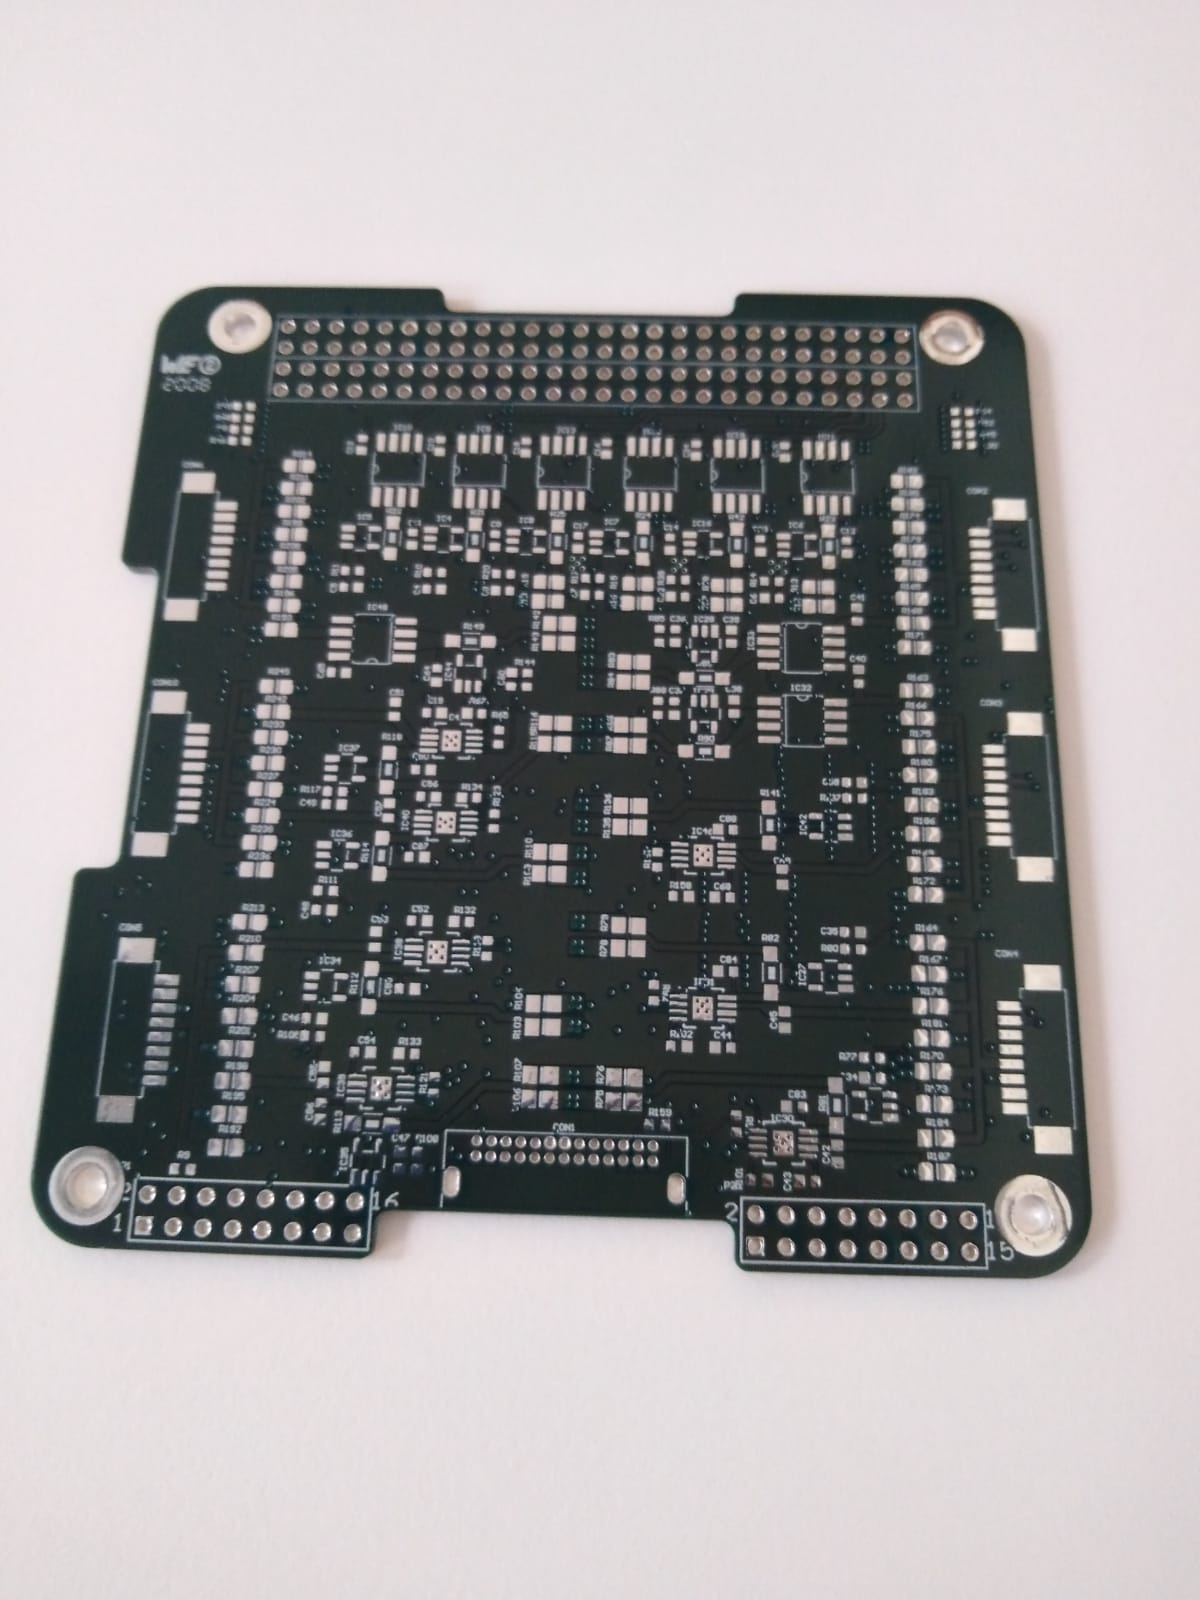
\includegraphics[scale=0.2]{PDU_PCB.jpeg}
	\caption{Power Distribution Board PCB}
	\label{fig: PCB_PDU}
\end{figure} 

\section{Physical Dimensions}

The PCB design rules such as board dimensions, max trace width, component-to-component distance, max vias size pad-to-pad distance are all contained within the German Orbital Systems templates and requirements, as well as the manufacturer requirements. 

The total thickness of the PCB is 1.7 mm. The PCB of the PDU has eight copper layers with 0.036 mm each. Every copper layer is separated with dielectric material FR-4 with thickness of 0.254 mm. FR-4 is a composite material typically composed of woven fiberglass with epoxy resin binder. 


\begin{figure}[h]
	\centering
	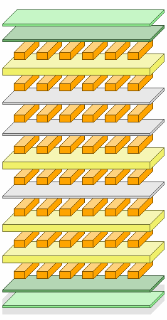
\includegraphics[scale=0.8]{layer1.png}
	\caption{Layer stack}
	\label{fig: layerstack}
\end{figure} 


The required PDU dimensions for the length and width are 90.16mm x 95.90mm. These dimensions are standardized by German Orbital Systems.

\section{Layout Design}

The layout design was started with the power trace width calculation.
According to the power requirements, maximum supplied current on the PDU for the Descartes Mission is 1.5A which has to be supplied to the Hispico S-band transceiver. The minimal width of the power lines on the PDU is no less than 1 mm. Due to the vacuum, the outer layers cannot lose heat during convection. Therefore, the K coefficient of traces is the same for the inner and outer layers.

The maximum current can be calculated by equation \ref{eq: amp}

\begin{equation}\label{eq: amp}
I = K \times dT^{0.44} \times (W \times H)^{0.725}
\end{equation}

Where\\

I - Max current\\
K - Coefficient for traces (0.024)\\
W - Width in mm(1)\\
H - Thickness in mm(0.036) \\
dT - Temperature rise above ambient in $^\circ$C(15)\\

As a result, maximum current that can be transfered through the track $\approx$ 1.5A.\\ 

The PCB  has eight copper layers. Top and bottom layers are used for power transmission, partially as a signal transmission and as a ground polygon. Second and the seventh layers are used for a signal transmission. The design of the second and seventh layers is designed so that the signal lines have a track width of 0.4 mm as straight as possible to reduce noise. The third and sixth layers are ground layers they are used for decoupling the signal layers as well as for a thermal dissipation reasons, which is an important function considering the fact that PDU board transfers power. Fourth and fifth layers are power layers, they consist of the power polygons which transfer power from the source to the integrated circuits and to the connectors.   

\begin{figure}[h]
	\centering
	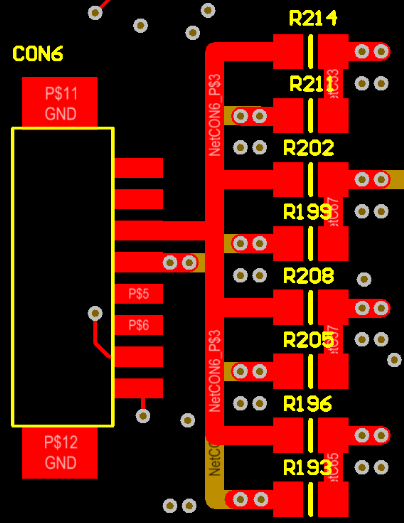
\includegraphics[scale=0.4]{resist_con.png}
	\caption{Zero ohm resistors to payload connector network}
	\label{fig: res}
\end{figure} 


Fig. \ref{fig: res} shows only top, middle power layers and top silk overlay of the PCB.

  
The main feature of the Power Distribution Board layout design is the flexibility of a choosing connector, power line and required voltage. PDU has an ability to set up the connector with the different switch power outputs.The PDU, as it was explained in the chapter \ref{sec:tech77}, uses two types of connectors: 9-pin connector and 8-pin connector. Each of those two types has a two input power pins for a power transmission.  Some connectors in the Descartes Mission required 2 inputs from two different switches such as connectors: K5, K6, K7 which have to transfer power to the DeCor payload. The connector designations are given in Appendix A. The zero ohm resistors allow to select the power channels that will supply power to the payload. Each payload connectors can be adjusted to receive power from one of the four load switches. Fig. \ref{fig: res} shows example of the connection layout design between zero ohm resistors and the payload connector. Zero ohm resistors are placed maximum close to the payload connector in order to make more space on the PCB. 

The load switches are located on the top and bottom side of the PCB. Each switch must supply power to a specific connector in order to reduce the length of the power path between the switch and  corresponding connector. The switches were located as close to their respective connectors as possible in order to reduce the path length and resistance, which directly affects the voltage drop. 

\begin{figure}[h]
	\centering
	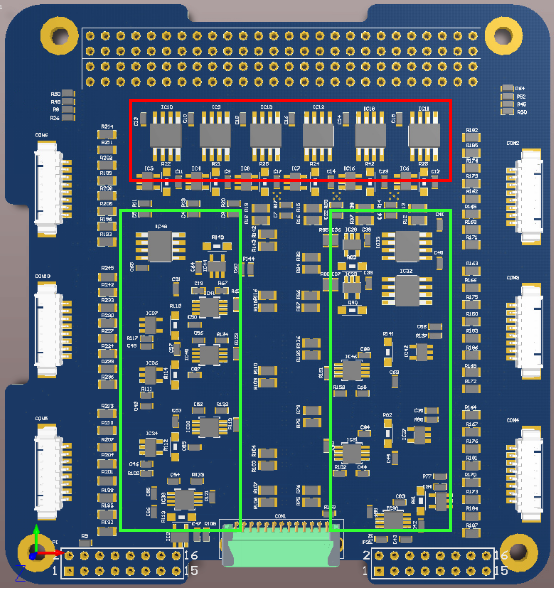
\includegraphics[scale=0.5]{pdu_top_3d_new.png}
	\caption{Top view of the PDU}
	\label{fig: toppducon}
\end{figure} 

Fig. \ref{fig: toppducon} shows the placement of the switches on the top layer of the PDU. Switches, responsible for a bus power line commutation are emphasized with a red frame. In order to decrease the distance between the load switches and PC104 connector, which are used to transfer bus power to oder boards in the stack, switches were located on the top side of the the PCB in a row. The payload switches, are emphasized with green frames, located on the left and right sides of the PCB. This allow them to transfer power without extra losses on the shortest distance to the relative payload connectors.



\begin{figure}[h]
	\centering
	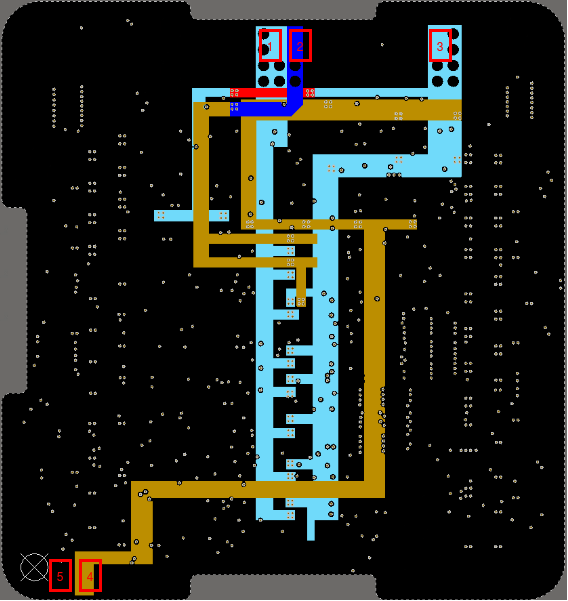
\includegraphics[scale=0.5]{polygons.png}
	\caption{Power polygons of the PDU}
	\label{fig: poly}
\end{figure} 

Fourth and fifth copper layers of the PCB are used to transfer a high power. One of the main tasks of the middle power layers is to transfer current from the source pads to the relative IC's via polygons. There are 5 main power source pads on the PCB: 7.4V, 3.3V BUS, 3.3V PAYL, 5V BUS, 5V PAYL. Figure \ref{fig: poly} illustrates the main power sources on the PCB, where:\\ \\
 1 - 5V PAYL\\
 2 - 3.3V PAYL\\
 3 - 7.4V\\
 4 - 5V BUS\\
 5  - 3.3V BUS\\

The minimum width of the polygons was calculated according to the formula \ref{eq: amp} and the maximum current with the coefficient of internal traces.

\begin{equation}
W = \frac{\sqrt[0.725]{\frac{1.5}{0.024 \times 15^{0.44}}}}{0.035}
\end{equation} 

According to the upper mention calculation, the minimal required inner width of the trace should be not smaller then 1.0 mm. The minimal width of the Power distribution board inner traces is 1.5 mm which within the required tolerance. 



\begin{figure}[h]
	\centering
	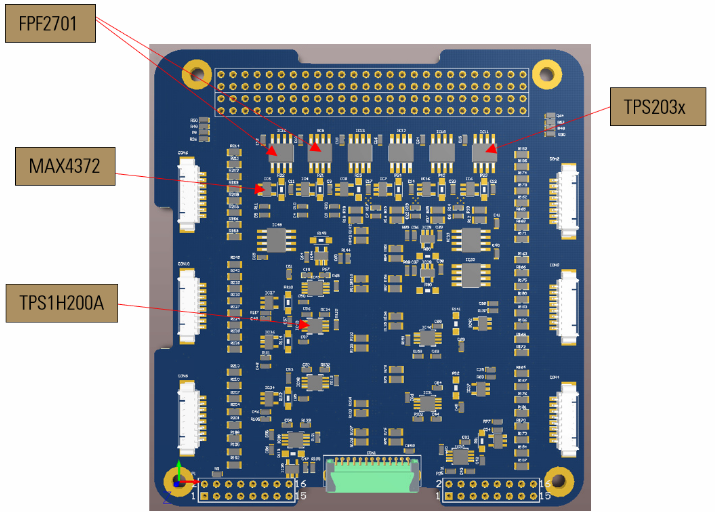
\includegraphics[scale=0.38]{pdu_top_component.png}
	\caption{Types of components on  top view of the PDU }
	\label{fig: pdu_comp_top}
\end{figure} 

\begin{figure}[h]
	\centering
	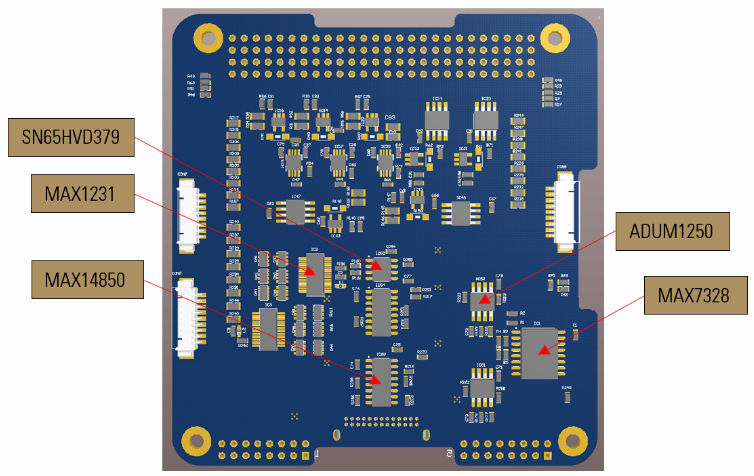
\includegraphics[scale=0.38]{pdu_bot_component.png}
	\caption{Types of components on  bottom view of the PDU}
	\label{fig: pdu_comp_bot}
\end{figure} 


Figures \ref{fig: pdu_comp_top} and \ref{fig: pdu_comp_bot} show placement of components on the PCB.
 


